\chapter{Experiments}
In this section, I will discuss how I evaluate the LSH with some real world data, and comparison with other spatial indexes. Finally, present the outcome that is measured from various aspects.

\section{Experimental Setup}

For evaluation, the LSPH is implemented in C++ and has been tested on a machine with 2.2GHz 6-core Intel Core i7 CPU and 16GB memory. 

\begin{center}
\begin{adjustbox}{max width={\textwidth}, max totalheight={\textheight},keepaspectratio}
\begin{threeparttable}
\caption{Datasets}

\begin{tabular}{c|c c c}
    \toprule
                        % & \multicolumn{3}{c}{Dataset} \\\midrule \midrule
    \textbf{Name}    &\textbf{Size}  & \textbf{No. of data pairs} & \textbf{Data type}             \\ \midrule 
    \texttt{post}    & 2.2M & 123,593             &Geographic Coordinates \\
    \texttt{g2}      & 18K  & 2,048               & Synthetic Clusters    \\
    \texttt{osm}     & 3.0G & 114,932,854         &Geographic Coordinates \\
     \bottomrule
\end{tabular}
% \begin{tablenotes}
% \item[1] qwerty; \item[2] asdfgh
% \end{tablenotes}
\end{threeparttable}
\label{table:datasets}
\end{adjustbox}
\end{center}

\subsection{Datasets} 
As shown in the Table \ref{table:datasets} above, we have two real world datasets the \texttt{post} \cite{rtreeportal} and \texttt{osm} \cite{OpenStreetMap}, and one synthetic dataset the \texttt{g2} \cite{G2sets}. 

\begin{itemize}
  \item \texttt{post}: The \texttt{post} dataset contains 123,593 coordinates of post offices across North America. The distribution of this dataset is more evenly.
  \item \texttt{g2}: The \texttt{g2} is a synthetic cluster dataset that contains 2,048 points that are computed from Gaussian clusters with 2 dimensions and the standard deviation set to 10. 
  \item \texttt{osm}: The dataset \texttt{osm} contains 114,932,854 coordinates in Australia and Oceania from OpenStreetMap. This dataset contains large amount of data points, and its distribution is highly skewed. 
\end{itemize}


\begin{figure}
    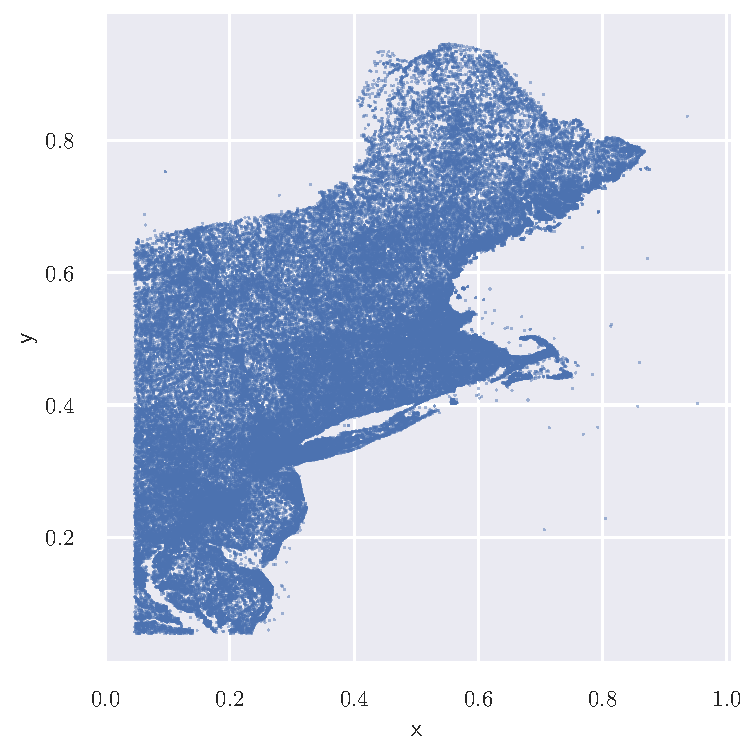
\includegraphics[width=.33\textwidth]{Figures/post_p.pdf}\hfill
    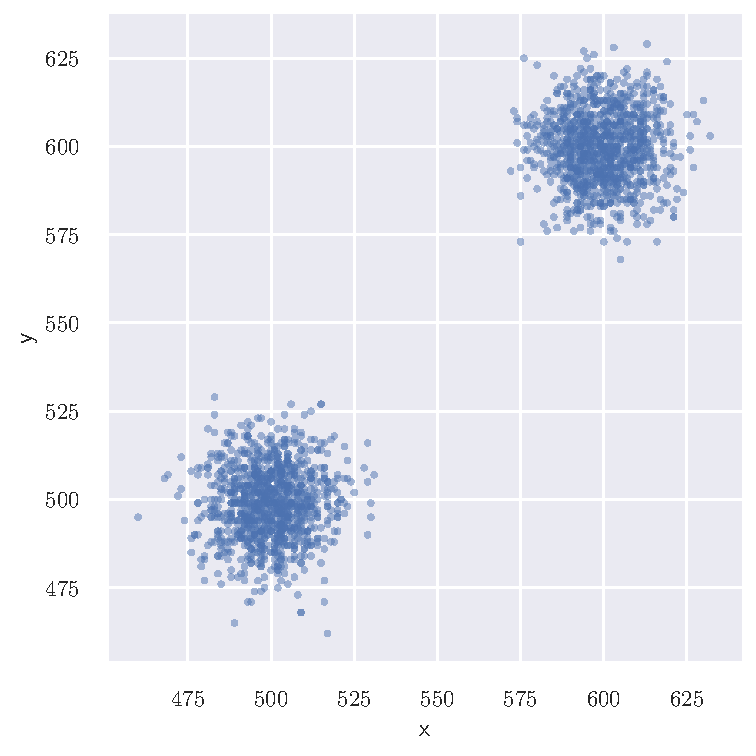
\includegraphics[width=.33\textwidth]{Figures/g2.pdf}\hfill
    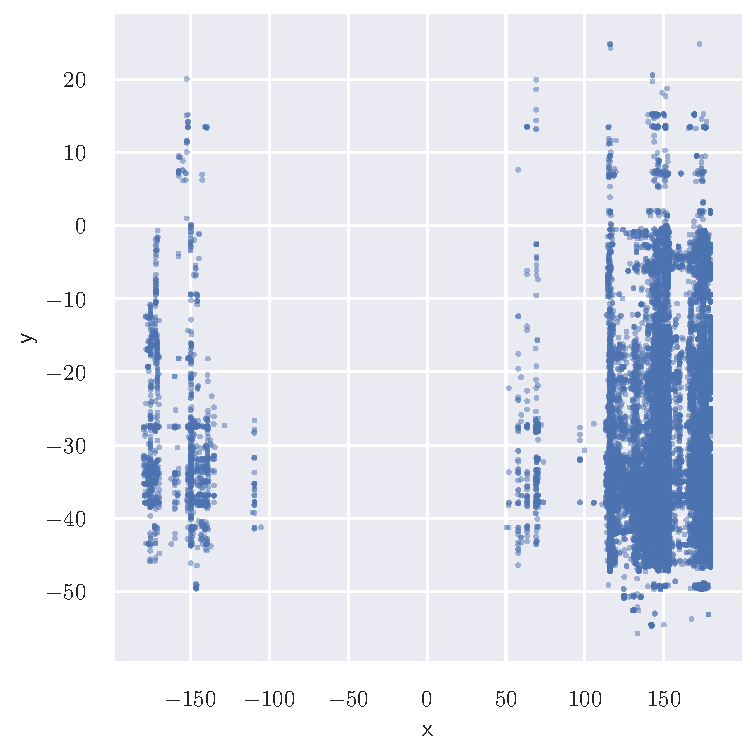
\includegraphics[width=.33\textwidth]{Figures/aus-ocean_p.pdf}
    \caption{Distribution of \texttt{post}, \texttt{g2} and \texttt{osm} datasets }\label{fig:datasets}
\end{figure}

Figure \ref{fig:datasets} illustrates the general size and distribution of each dataset. The three datasets represent three different data distribution settings: the post dataset has relatively uniform data distribution, and with over 100,000 data points making it common scenarios for spatial data indexing; the g2 is a synthetic two-dimensional dataset contains two clusters of data points, which is skewed on the both of axis, to test the skewness handling among the indexes; the osm is another real-world dataset with a sizable amount of data, and combine the heavily skewed data distribution, to test the performance under skewed high volume real-world scenario.  



\subsection{Competitors}
We are comparing LSPH with one traditional spatial index \textbf{R-Tree} \cite{Guttman:1984ka} and one learned spatial index \textbf{ZM} \cite{Wang:2019ks}

\textbf{R-Tree}: A templated C++ version implemented by Greg Douglas \cite{rtreecplus} is used for comparison. The partitioning method in this version uses the Quadratic-Cost splitting algorithm from the original R-Tree paper \cite{Guttman:1984ka}. 

\textbf{Learned ZM index}:  For the ZM model, the two-dimensional datasets convert to 64-bit one-dimensional data, using the Z-order curve transformation. We use an RMI implementation from the author of RadixSpline and SOSD \cite{Kipf:2020wr, sosd}. 

\subsection{Evaluation Metrics}
We measure the performance of all indexes from four aspects: memory consumption during runtime, time cost of index building, time cost of query and accuracy of the query result. The runtime memory reflects the space complexity of the index method, and the measurement is using the Linux command \texttt{time -v} to get the maximum resident set size of allocated memory size during runtime. Time measurements in the experiment were using the C++ \texttt{std::chrono} library to record the time during index building and query execution in nanoseconds. 

In the experiment, we use sorted arrays to build all indexes. Each index takes two data values as a pair of keys for lookup query, and if it exists in the index, the returned results should match with the query keys. We execute the lookup query overall key pairs in all three datasets. Note that there are some duplicates in the dataset, and they have been filtered out before indexes building. Therefore, the input number of the query should match with the returned results if the index can locate the key without errors. 



\section{Performance Results}

\begin{figure}
    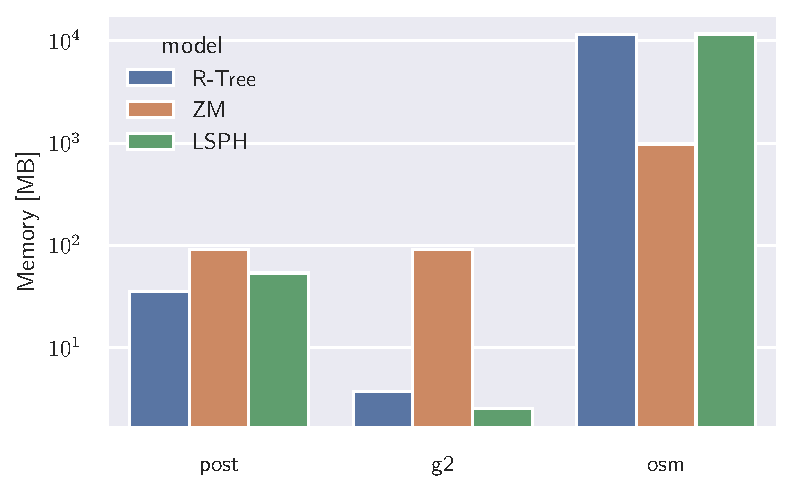
\includegraphics[width=.5\textwidth]{Figures/memory.pdf}\hfill
    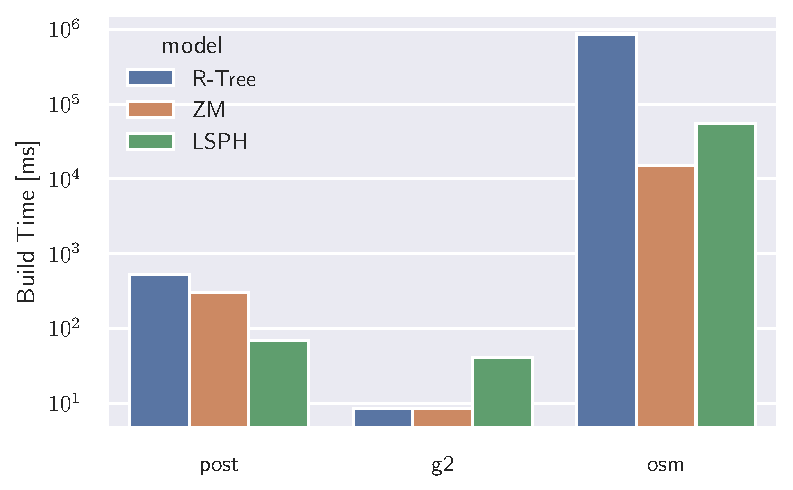
\includegraphics[width=.5\textwidth]{Figures/build_time.pdf}
    \\[\smallskipamount]
    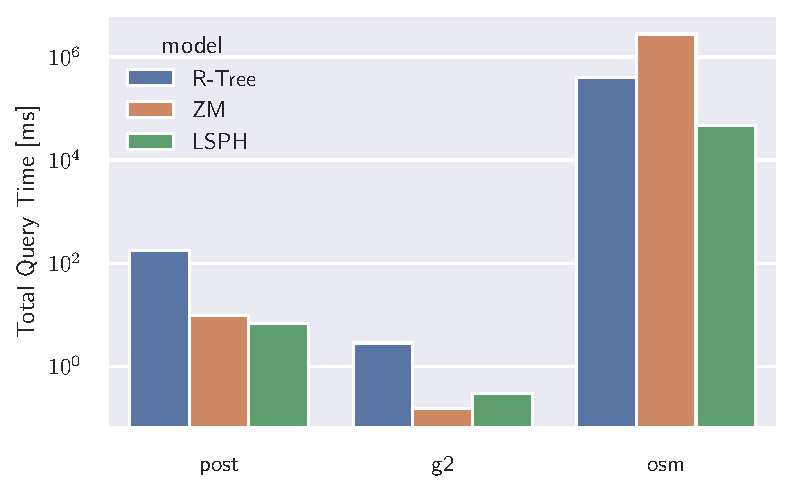
\includegraphics[width=.5\textwidth]{Figures/query_time.pdf}\hfill
    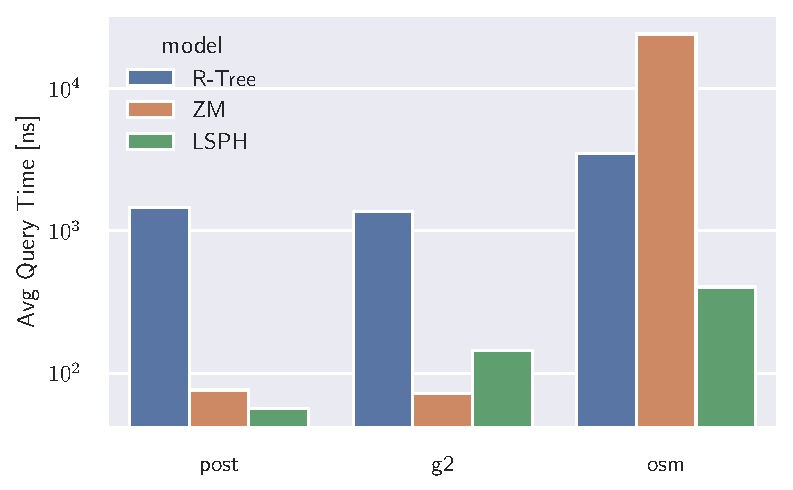
\includegraphics[width=.5\textwidth]{Figures/avg_query_time.pdf}
    \caption{Point query performance comparison on runtime memory, build time, total query time and average query time for all three spatial indexes}\label{fig:performance}
\end{figure}



\textbf{Overall performance}: We first compare the point query performance of all indexes on three datasets. Figure \ref{fig:performance} illustrates the overall performance of all indexes. The local search in the last step search in ZM used binary search, the total query time record the search range produced by a linear model plus the binary search execution time.  R-Tree uses minimum  bounding boxes to store all spatial objects. Therefore, for the point query in R-Tree, we set the minimum point and maximum point of a bounding box as the same pair of data values. As we see from the result, the LSPH has several advantages in memory and lookup query performance under certain conditions. 


\textbf{Runtime Memory}:
Comparing our method with R-Tree and ZM in terms of runtime memory consumption, as shown in the top-left diagram in Figure \ref{fig:performance}. LSPH consumes a similar amount of memory as R-Tree for all three sets of data. ZM costs more memory than LSPH and R-Tree in the \texttt{post} and \texttt{g2} dataset but costs less in the \texttt{osm} dataset. The ZM implementation requires running a rust code and converting it into C++ code, so it might consume more during conversion. The increase of numbers in the dataset causes a consistent growth in LSPH and R-Tree. For ZM, the memory cost is maintained at a certain level without concerning too much on the dataset size. 


\textbf{Build Time}: The build time of LSPH on a uniformly distributed dataset is outperforming the other two indexes. However, it cost more on skewed dataset \texttt{g2} and \texttt{osm}. Since we are using a linear model for the ZM, the build time is much faster than as if we were training a neural network. The reason for the slower build time of LSPH on the skewed dataset is that skewed data creates more chaining in the hashmap, which increases the node access during insertion. 



\textbf{Query Time}: Lookup query time showed a lookup performance advantage of LSPH. Note the log time scale in the total query time on the bottom of Figure \ref{fig:performance}, we also add an average query time for comparison. LSPH performed the best out of three indexes in the \texttt{post} and \texttt{osm}, and second place in the \texttt{g2}. The lookup speed in LSPH performs best in uniformly distributed datasets, it even can reach exact $O(1)$ if in a perfectly distributed dataset. The skewed data creates linked list overflow that causes some performance drop, but the average lookup speed is still kept at a slower growth compared to the ZM. Although the lookup speed is much slower on an extreme cluster case that values on both axes are skewed, the LSPH still does a better job than ZM in terms of accuracy, which will be discussed in the next section.   


\textbf{Accuracy}


\begin{center}
\begin{adjustbox}{max width={\textwidth}, max totalheight={\textheight},keepaspectratio}
\begin{threeparttable}
\caption{Point Query Accuracy}
\begin{tabular}{c|c c c}
    \toprule
                        % & \multicolumn{3}{c}{Dataset} \\\midrule \midrule
        &\textbf{R-Tree}  & \textbf{ZM} & \textbf{LSPH}             \\ \midrule 
    \texttt{post}    & 100\% & 99.99\% & 100\% \\
    \texttt{g2}      & 100\% & 99.71\% & 100\%  \\
    \texttt{osm}     & 100\% & 96.84\% & 100\% \\
     \bottomrule
\end{tabular}
% \begin{tablenotes}
% \item[1] qwerty; \item[2] asdfgh
% \end{tablenotes}
\end{threeparttable}
\label{table:accuracy}
\end{adjustbox}
\end{center}



\subsection{Range Query Performance}
\begin{figure}
    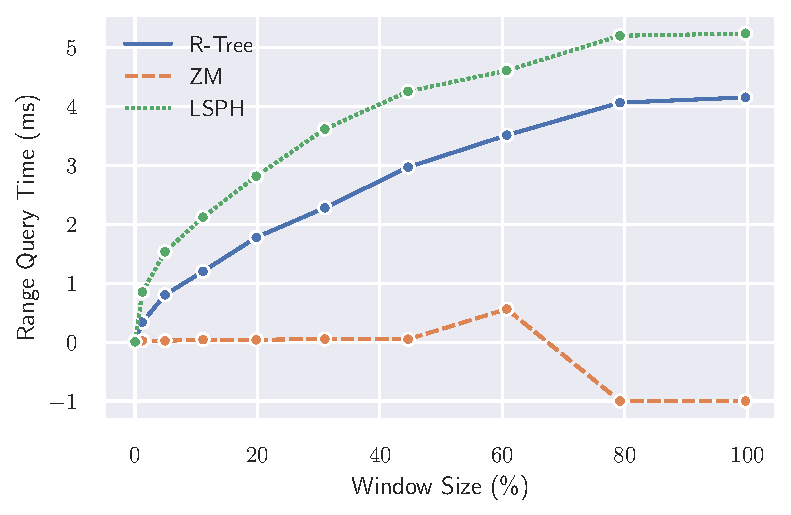
\includegraphics[width=\textwidth]{Figures/range_result.pdf}\hfill
    \caption{Range Query performance on dataset \texttt{post}. The window size is corresponding to the query selectivity, which is between 0.0-100.0\%. The -1 in ZM represents the return results are out of search range.}\label{fig:range_result}
\end{figure}